Os métodos de Newton se baseiam em encontrar uma aproximação quadrática $ q(x) $ a partir do teorema de Taylor para a função objetivo $ f(x) $, e assim, encontrar o seu mínimo.
	
	\begin{quote}
		\centering
		Lei de Iteração:
	\end{quote}
	
	\begin{equation}
		x^{k+1} = x^k - [G^k]^{-1}g^k
	\end{equation}

Teoricamente, a vantagem do método de Newton em relação aos outros é que, para funções quadráticas, ele converge em apenas uma iteração. Porém, um dos problemas do método é ele ser de segunda ordem, o que significa que ele depende tanto do valor da hessiana quanto do gradiente da função objetivo, e alguns casos, a convergência pode ser comprometida devido ao fato de que a hessiana em um dado ponto pode não ser positiva definida.

Depois de construído o algoritmo, foram testadas quatro funções para efeitos de comparação:

\begin{itemize}
	\item $ f_1(x,y) = x^2 + y^2$
	\item $ f_2(x,y) = -e^{-x^2 -y^2}$
	\item $ f_3(x,y) = cos(\frac{xy}{5})+sin(\frac{xy}{5}) $
	\item $ f_4(x,y) = |x+y| $
\end{itemize}

\newpage

\begin{figure}[H]
	\begin{center}
		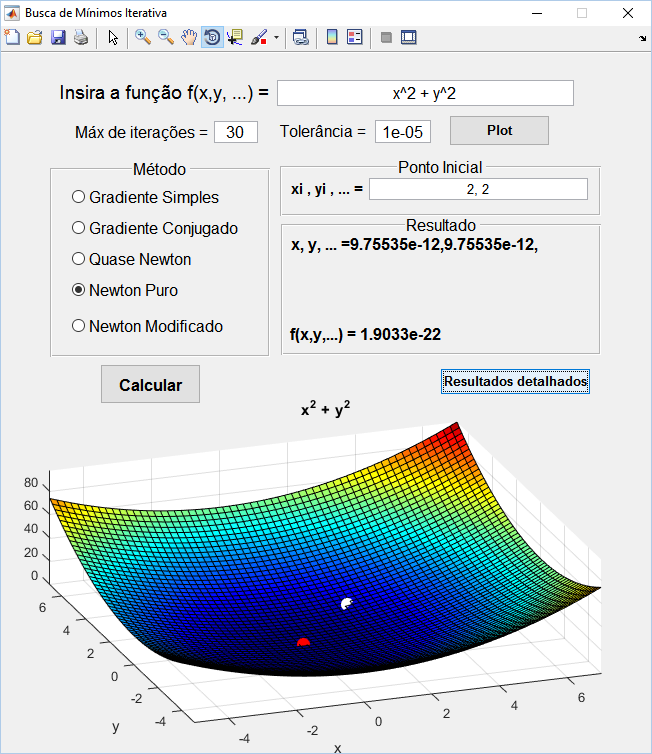
\includegraphics[width=12cm]{../newton/f1_gui}   
		\caption{Janela de inicialização de $ f_1(x,y) $}
		\label{fig:newton_f1_gui}
	\end{center}
\end{figure}

\begin{figure}[H]
	\begin{center}
		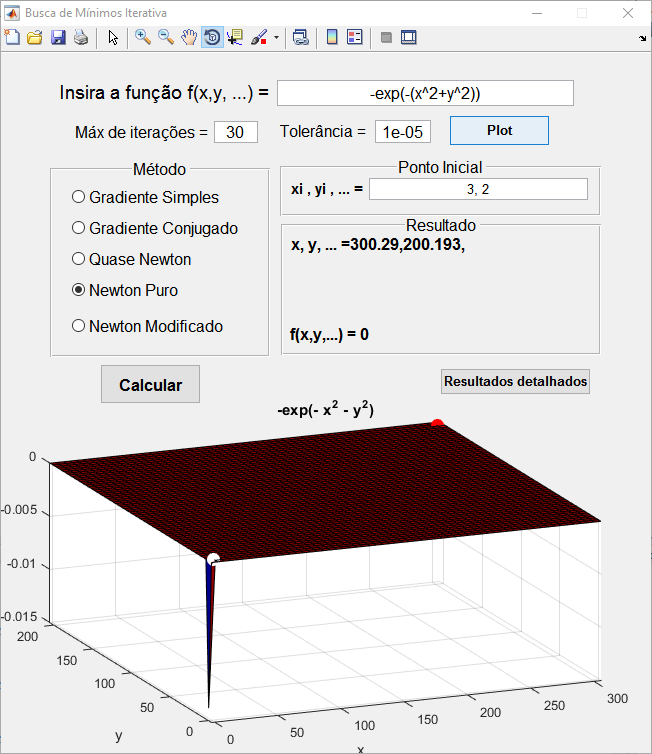
\includegraphics[width=12cm]{../newton/f2_gui}   
		\caption{Janela de inicialização de $ f_2(x,y) $}
		\label{fig:newton_f2_gui}
	\end{center}
\end{figure}

\begin{figure}[H]
	\begin{center}
		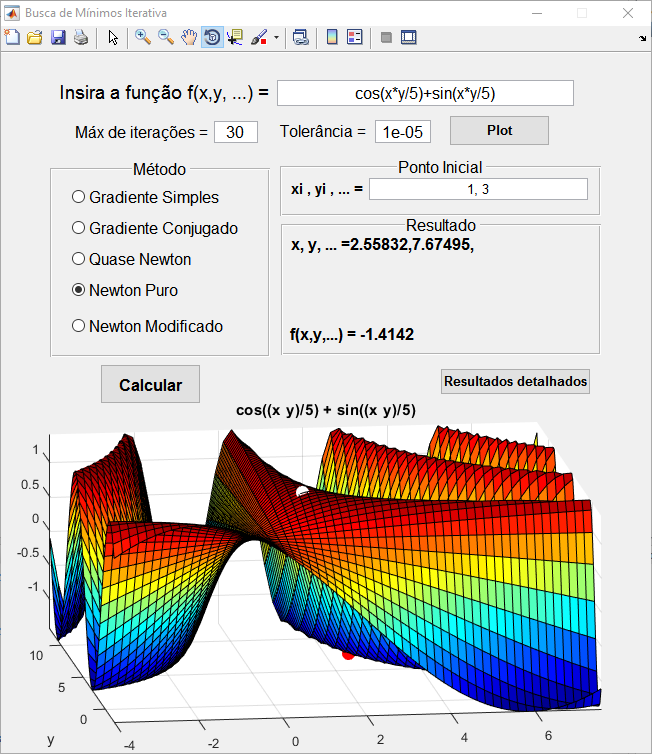
\includegraphics[width=12cm]{../newton/f3_gui}   
		\caption{Janela de inicialização de $ f_3(x,y) $}
		\label{fig:newton_f3_gui}
	\end{center}
\end{figure}


\begin{figure}[H]
	\begin{center}
		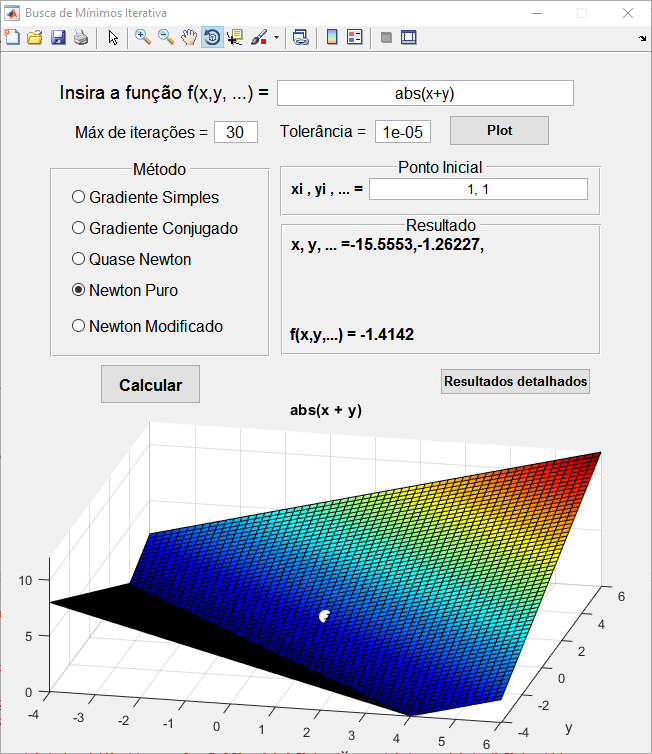
\includegraphics[width=12cm]{../newton/f4_gui}   
		\caption{Janela de inicialização de $ f_4(x,y) $}
		\label{fig:newton_f4_gui}
	\end{center}
\end{figure}
